\subsection{Camera Testing}
After obtaining two of the MT9V034 cameras chosen through the process referenced in Appendix item \ref{camdecision}, several steps were taken to obtain test data from each camera. These steps are outlined in the following sections.

\subsubsection{Camera Operation}
In order to gather working images from each camera module, we first needed to understand what circuitry our camera module breakouts contained so that we could interface with them. MT9V034 camera breakouts were purchased from Leopard Imaging Inc. Although these camera module breakout boards are intended to be used with Leopard Imaging's LeopardBoard ARM development board, the breakouts were found to contain only the supporting circuitry recommended in the MT9V034 datasheet, and we decided that they would be ideal for our application \cite{livm34lp,mt9v034}. 
\par
Once the schematics of each camera module breakout were known, it was then possible to design a basic control interface for each camera. According to the MT9V034 datasheet, each camera module needs to be supplied with an external Master Clock and Output Enable signal in order to operate \cite{mt9v034}. A simple Verilog module for the Nexys3 Spartan-6 FPGA board was created in order to supply the camera module with a 24MHz master clock signal, and a switch was used to toggle output enable. With this module implemented, the camera module's default outputs could then be observed. In order to interface the camera module with an FPGA, the breakout board shown in Figure \ref{camBreakoutBoard} was also created to make the module's pins more easily accessible based on functionality. 

\begin{figure}[H]
	\centerline{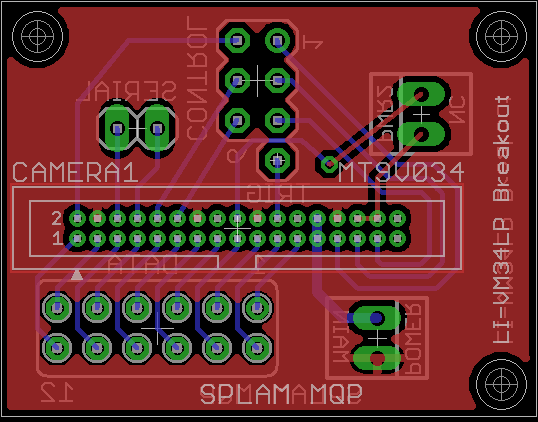
\includegraphics[width=0.5\textwidth]{camera_board.png}}
	\caption{LI-VM34LP Breakout Board}
	\label{camBreakoutBoard}
\end{figure}

\par
By default, the MT9V034 camera module will continuously gather image data at 60Hz  as long as it is supplied with an external clock signal and output is enabled \cite{mt9v034}. Several output signals from the camera module are then used to transmit image data. Each image, or frame, is broken up into individual "lines" which correspond to a line of pixels that stretch the width of the frame. Since our camera module captures images at 752x480 pixel resolution, one frame will contain 480 lines of 752 pixels each. The camera module breaks up image data by frame and line, and camera data pins FRAME\_VALID and LINE\_VALID are toggled to indicate the transmission of a frame or line. The timing diagram shown in Figure \ref{FvLv} shows the operation of these pins while transmitting an image.

\begin{figure}[H]
	\centerline{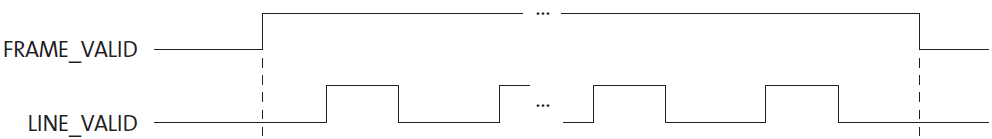
\includegraphics[width=1.0\textwidth]{camFvLv.png}}
	\caption{Frame and Line Valid \cite{mt9v034}}
	\label{FvLv}
\end{figure}

\par
Since the MT9V034 module transmits image data in parallel and each pixel contains 10 bits of resolution, 10 pins are used to transmit pixel values in parallel. Pixel data is transmitted in correspondence with LINE\_VALID and output clock signal PIXCLK. When LINE\_VALID is asserted, the pixel data pins are updated with values corresponding to pixels 0-751 of the given line. Values for each pixel are written out on the falling edge of the camera's PIXCLK pin, allowing for each pixel's value to be read on the rising edge of PIXCLK cycle. A full LINE\_VALID data transmission sequence will therefore contain 752 PIXCLK cycles, corresponding to the 752 pixels that make up the given line. A timing diagram of this data transmission scheme is shown in Figure \ref{LvDout}.  
\begin{figure}[H]
	\centerline{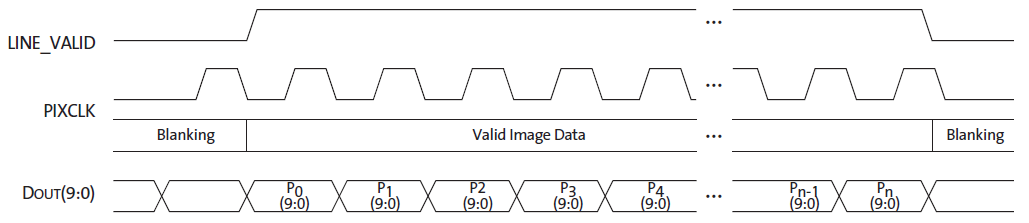
\includegraphics[width=1.0\textwidth]{camLvPckDout.png}}
	\caption{Line Data Transfer \cite{mt9v034}}
	\label{LvDout}
\end{figure}

\par
The default camera data transmission scheme was also examined using an oscilloscope, as shown in Figure \ref{camDataTransfer}, with channels 1-4 corresponding to camera PCLK, FRAME\_VALID, LINE\_VALID, and Data[0], respectively. In the case of Figure \ref{camDataTransfer}, the camera is initially powered off, resulting in an inactive PCLK signal.
\begin{figure}[H]
	\centerline{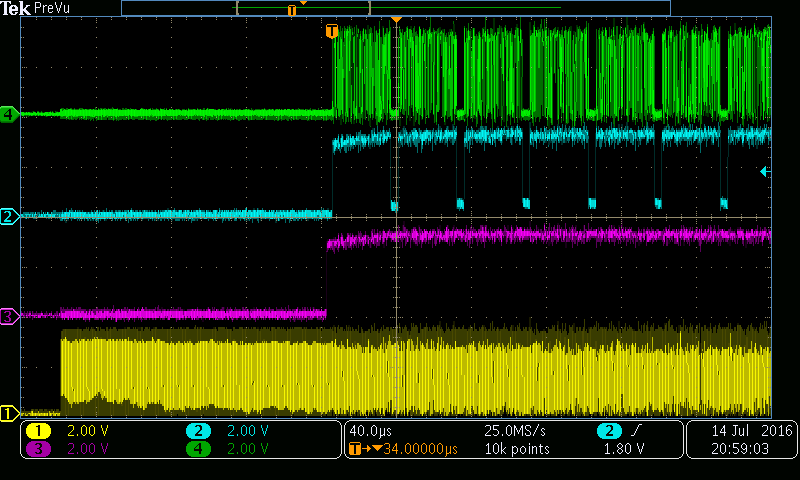
\includegraphics[width=1.0\textwidth]{oScope/pclk_fv_lv_data2/tek00004.png}}
	\caption{Camera Data Transfer}
	\label{camDataTransfer}
\end{figure}

\subsubsection{I$^2$C Control} 
The MT9V034 Camera module's mode of operation can be configured using a standard I$^2$C control interface. I$^2$C, or Inter-Integrated Circuit, is a bidirectional serial interface that allows for a master device to read from and write to several slave devices sharing the same data bus. An I$^2$C interface will use a Serial Data Line (SDA) and Serial Clock Line (SCL) that are normally pulled to 5V. When one connected I$^2$C device wishes to communicate with another, it will pull the SDA line low while leaving the SCL line high. The master device will then begin clocking the SCL line, and SDA will be used to transfer 7 bits representing the address of the desired slave device, along with an 8th bit representing whether it would like to read or write to the device. An example of this transfer is shown in Figure \ref{I2Cexample}. A second 8 bit sequence representing a specific register within the slave device may also be transmitted with the device address. For example, if the master device wishes to write to slave device 0x40 at register 0x00, it will transmit 0x41 (address 0x40 and WRITE), followed by 0x00. If the slave device receives this transmission, it will acknowledge by pulling the SDA line low. At this point, the master can then transmit the value that it wishes to write to the given slave address and register. If the operation were a read rather than a write, the slave would transmit a value back to the master.  
\par
\begin{figure}[H]
	\centerline{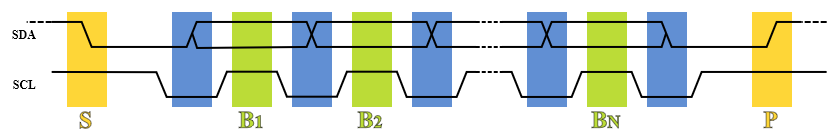
\includegraphics[width=1.0\textwidth]{I2C_data_transfer.png}}
	\caption{Example I$^2$C Data Transfer}
	\label{I2Cexample}
\end{figure}

Based on the LIVM34LP camera breakout schematic, the camera breakout boards have been configured so that each camera is accessible at I$^2$C address 0x58 \cite{livm34lp}. Note that since both cameras come configured with the same I$^2$C bus address, a pullup resistor must be added to one of the cameras I$^2$C address lines so that both are individually accessible on a shared bus.
\par
Although the MT9V034 camera control registers are closed source, the previous model's registers are available in the camera module datasheet, and have been found to work with the current model thus far \cite{mt9v032}. As a baseline, the camera module was sent a read request at address 0x00, which should return 0x1324 for the MT9V034 camera module. An oscilloscope screenshot of this request is shown in Figure \ref{camVersion}, with the first packet consisting of a request to address 0x00 of device 0x058, and the second packet consisting of the camera's response of 0x1324. 
\begin{figure}[H]
	\centerline{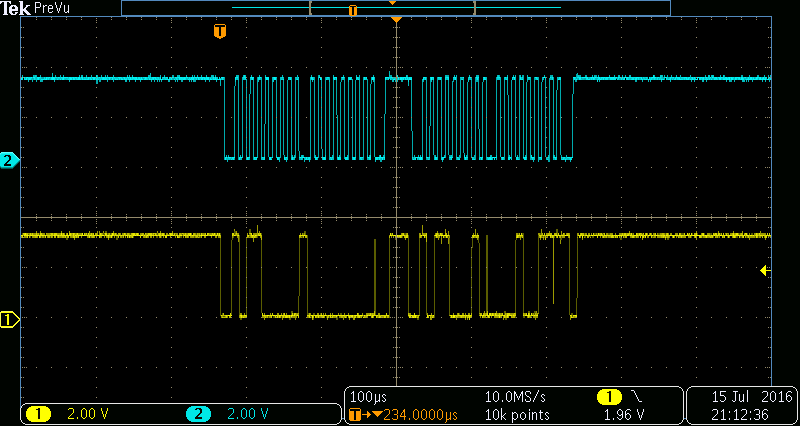
\includegraphics[width=1.0\textwidth]{oScope/i2c_0x00/tek00001.png}}
	\caption{Example I$^2$C Transfer with Camera}
	\label{camVersion}
\end{figure}

\par
After the camera I$^2$C was confirmed to work, the camera control register was modified to put the camera in "snapshot" mode. In this mode, the camera module will no longer continuously take pictures, and will only gather new images when an external trigger is activated. This is the mode that the camera will need to operate in in order to acquire stereo imagery, since a shared trigger line will allow for both cameras to be controlled simultaneously.
\par
According to the previous camera iteration's datasheet, the camera module's operational mode can be set through control register 0x07. By default, this register will be set to a value of 0x0388, which corresponds to master mode with parallel output and simultaneous readout of pixel data enabled \cite{mt9v032}. In order to put the camera in trigger mode, the control register needs to be written with value 0x0198, which allows for the same functionality as before with the exception of having continuous shutter mode replaced with an external trigger. For reference, a table with bit descriptions for the camera control register can be found in Appendix item \ref{camctlreg} \cite{mt9v032}.
\par
After modifying the state of this register, a button was attached to the camera's TRIGGER input line, and the TRIGGER and FRAME\_VALID lines were observed on channels one and two of the oscilloscope, as shown in Figure \ref{camInTrigMode}. This oscilloscope screenshot can be seen as an example of how the camera is no longer in continuous operation, since FRAME\_VALID only asserts itself in response to a TRIGGER input. 
\begin{figure}[H]
	\centerline{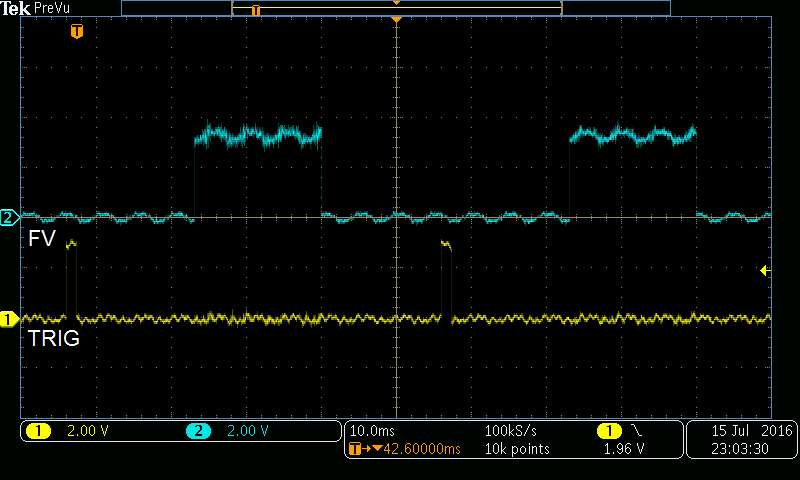
\includegraphics[width=1.0\textwidth]{oScope/i2c_0x07/externalTrigger/externalTrig.png}}
	\caption{Camera Trigger and FV in Trigger Mode}
	\label{camInTrigMode}
\end{figure}

\subsubsection{Data Management}
After successfully creating a camera control interface and placing the MT9V034 camera module in trigger mode, it was then possible to begin viewing images from the module. Since each image contains 752x480 pixels with 10 bits of resolution per pixel, a full camera image will consume 3,609,600 bits, or 440.6kB, as shown in Equation \ref{imagesize}.
\begin{equation} \label{imagesize}
Image\,\,Size = 752px*480px*10\frac{bits}{pixel} = 3609600\,bits*\frac{1\,byte}{8\,bits}*\frac{1 kB}{1024\,bytes} = 440.625kB
\end{equation}
\par
In order to send a camera image to a computer or monitor for viewing, several steps need to be taken. Although it would be ideal to transfer the image directly from the camera to a computer or display, this would be difficult to achieve due to the high speeds of the camera's data output. In order to properly synchronize camera data with a VGA display, both the camera and VGA display would have to run at exactly the same clock speed, and would need to have the same amount of vertical and horizontal blanking to display each pixel in its correct location. If the image were transferred to a computer, the act of packaging the information so that it may be interpreted by a computer would place severe limitations on the speed of the system. A proper solution to these timing issues would be to buffer the image between the camera and the desired output source, since this would allow for separate clock domains to be used for camera data transfer and data output. However, the act of locally buffering a camera image on an FPGA would also be difficult due to low memory resources. 
\par
Although 440kB may seem like a relatively small image size, creating a buffer object large enough for storing said image would consume an extremely large amount of logic. For reference, a standard Nexys3 FPGA evaluation board contains only 18kB of onboard Block RAM, and would not be able to buffer an image of this size without the use of external RAM \footnote{Xilinx, \textit{Spartan-6 FPGA Block RAM Resources}, 11.\\  \url{http://www.xilinx.com/support/documentation/user_guides/ug383.pdf}}. This leaves the final option of using either external RAM or a First-In First-Out (FIFO) memory array for transferring a captured image between clock domains. During initial development, an AL422B FIFO IC was used, since the IC has been created specifically for buffering VGA imagery similar to that of the MT9V034 camera module, and can be connected directly to the camera module outputs \cite{al422b}. The AL422B FIFO module contains 3M-bits of RAM that can be written to and read from in parallel, and supports separate input and output clock speeds between 1-50MHz \cite{al422b}. This means that the camera module can independently write pixel data to the FIFO as long as it operates at a speed between 1 and 50MHz, and the FPGA can read from the FIFO at any speed within the same range. Note that since this FIFO supports only 8-bit parallel data in and out, the lowest two bits of camera pixel data must be truncated. This isn't a major issue, since the truncation will correspond to a 4/1024 reduction in the range of values that each pixel can map to.
\par
With the inclusion of the external FIFO module, it is now possible to capture and store an image for future reading, and to read out image data in chunks. Keeping this in mind, the system shown in Figure \ref{camTestBDG} was created for transmitting camera images to a computer for external analysis. In order to reduce development time, an external microcontroller was used for controlling the camera module's I$^2$C interface and placing the module in trigger mode. Various buttons and switches on the FPGA were then used for controlling the camera output and trigger, allowing for a user to trigger an image for storage on the AL422B FIFO. Once the image has been stored on the FIFO, the FPGA is capable of reading the image line-by-line into an internal buffer. An internal System on Chip (SoC) is used to control FPGA reads from the FIFO into this internal buffer. An image dump will begin when the internal microcontroller signals to the FPGA to read a new line of pixels into its internal 1x752 pixel buffer. The FPGA will then signal to the microcontroller when this buffer has been filled, and the microcontroller will print out the value of each pixel in the buffer over UART. When the microcontroller finishes printing out the value of each pixel in the line buffer, it will signal to the FPGA to read in a new line of pixels. This process will repeat for each of the 480 lines of pixels in the image, allowing for the transmission of an entire image's worth of data. The Verilog implementation of the top module and line buffer for this camera interface can be found in Appendix item \ref{mt9v034TestCode}.

\begin{figure}[H]
	\centerline{\includegraphics[width=1.0\textwidth]{camTestBlockDiag.png}}
	\caption{Camera Test System Block Diagram}
	\label{camTestBDG}
\end{figure}
\par
An example of the transmission of one line of pixel data from the FIFO to the FPGA is shown in Figure \ref{fifoDataOut}.  The green, purple, blue, and yellow lines in this image represent pixel data, FIFO read enable, read reset, and read clock, respectively. Since the FPGA reads in one line of pixel data at a time, this process will take 752 read clock cycles, as measured in Figure \ref{fifoDataOut}. In order to simplify debugging, an internal counter and seven-segment display controller have also been implemented on the FPGA, and will display a running count of the number of pixel lines that have been read into the FPGA's internal buffer, ranging from 0x0000-0x01E0 (0-480). 
\begin{figure}[H]
	\centerline{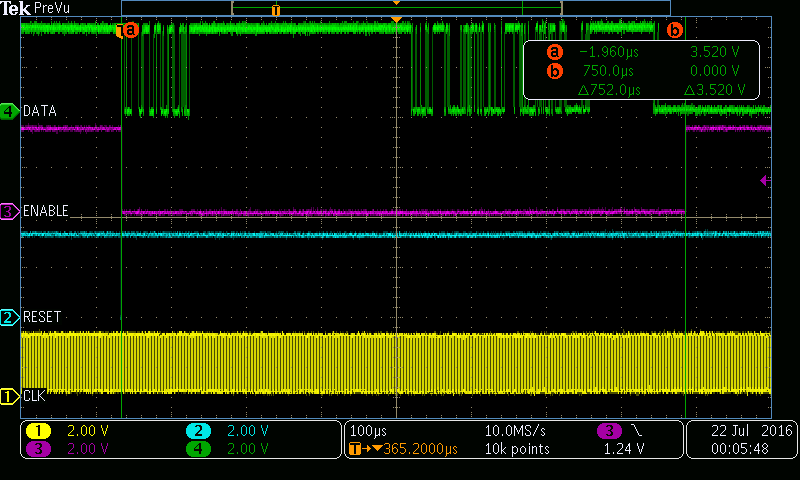
\includegraphics[width=1.0\textwidth]{oScope/camera_fifo/fifo_rstAndDataTimed.png}}
	\caption{Transferring Line Data from FIFO to FPGA}
	\label{fifoDataOut}
\end{figure}

\subsubsection{Transmitting Images Over UART for Analysis}
The source code found in Appendix item \ref{camTestC} was implemented on a Microblaze MCS in order to transmit camera line data from the FPGA's internal line buffer over UART. An example of the microcontroller's UART output is shown in Figure \ref{PuTTYfifoData}. The microcontroller will print the value of each pixel followed by a newline and carriage return, starting with the top left pixel in the acquired image. 
\begin{figure}[H]
	\centerline{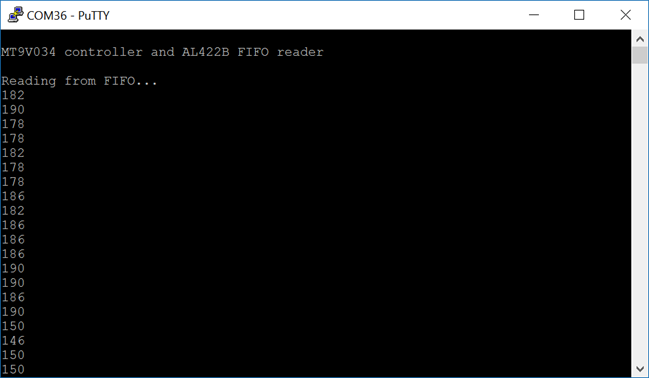
\includegraphics[width=0.8\textwidth]{oScope/camera_fifo/PuTTy.png}}
	\caption{Reading FIFO Data}
	\label{PuTTYfifoData}
\end{figure}
\par
After the image is recieved through PuTTy, the \textsc{Matlab} script found in Appendix item \ref{camTestMatlab} was used to parse the corresponding logfile into a greyscale image. An example image created through this process is shown in Figure \ref{notebookImage}. Note that the sub-optimal quality of this image is due to signal interference and degradation in the test setup's long wiring, as shown in Figure \ref{camTestSetup}. 
\begin{figure}[H]
	\centerline{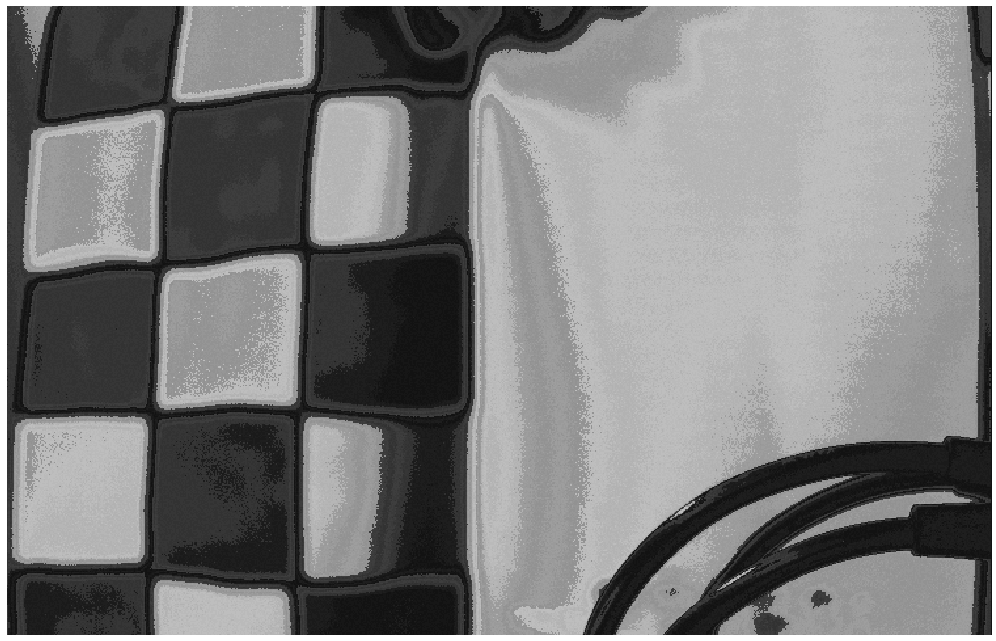
\includegraphics[width=0.75\textwidth]{oScope/camera_fifo/notebook.png}}
	\caption{Notebook With Grid and Oscilloscope Leads}
	\label{notebookImage}
\end{figure}
\par
Note that although this system was tested using the Nexys3 Spartan-6 FPGA board, the use of an external FIFO and little to no platform-specific hardware make it so that it can easily be implemented on any system, including the Zynq family of processors used on the ZedBoard.   
\begin{figure}[H]
	\centerline{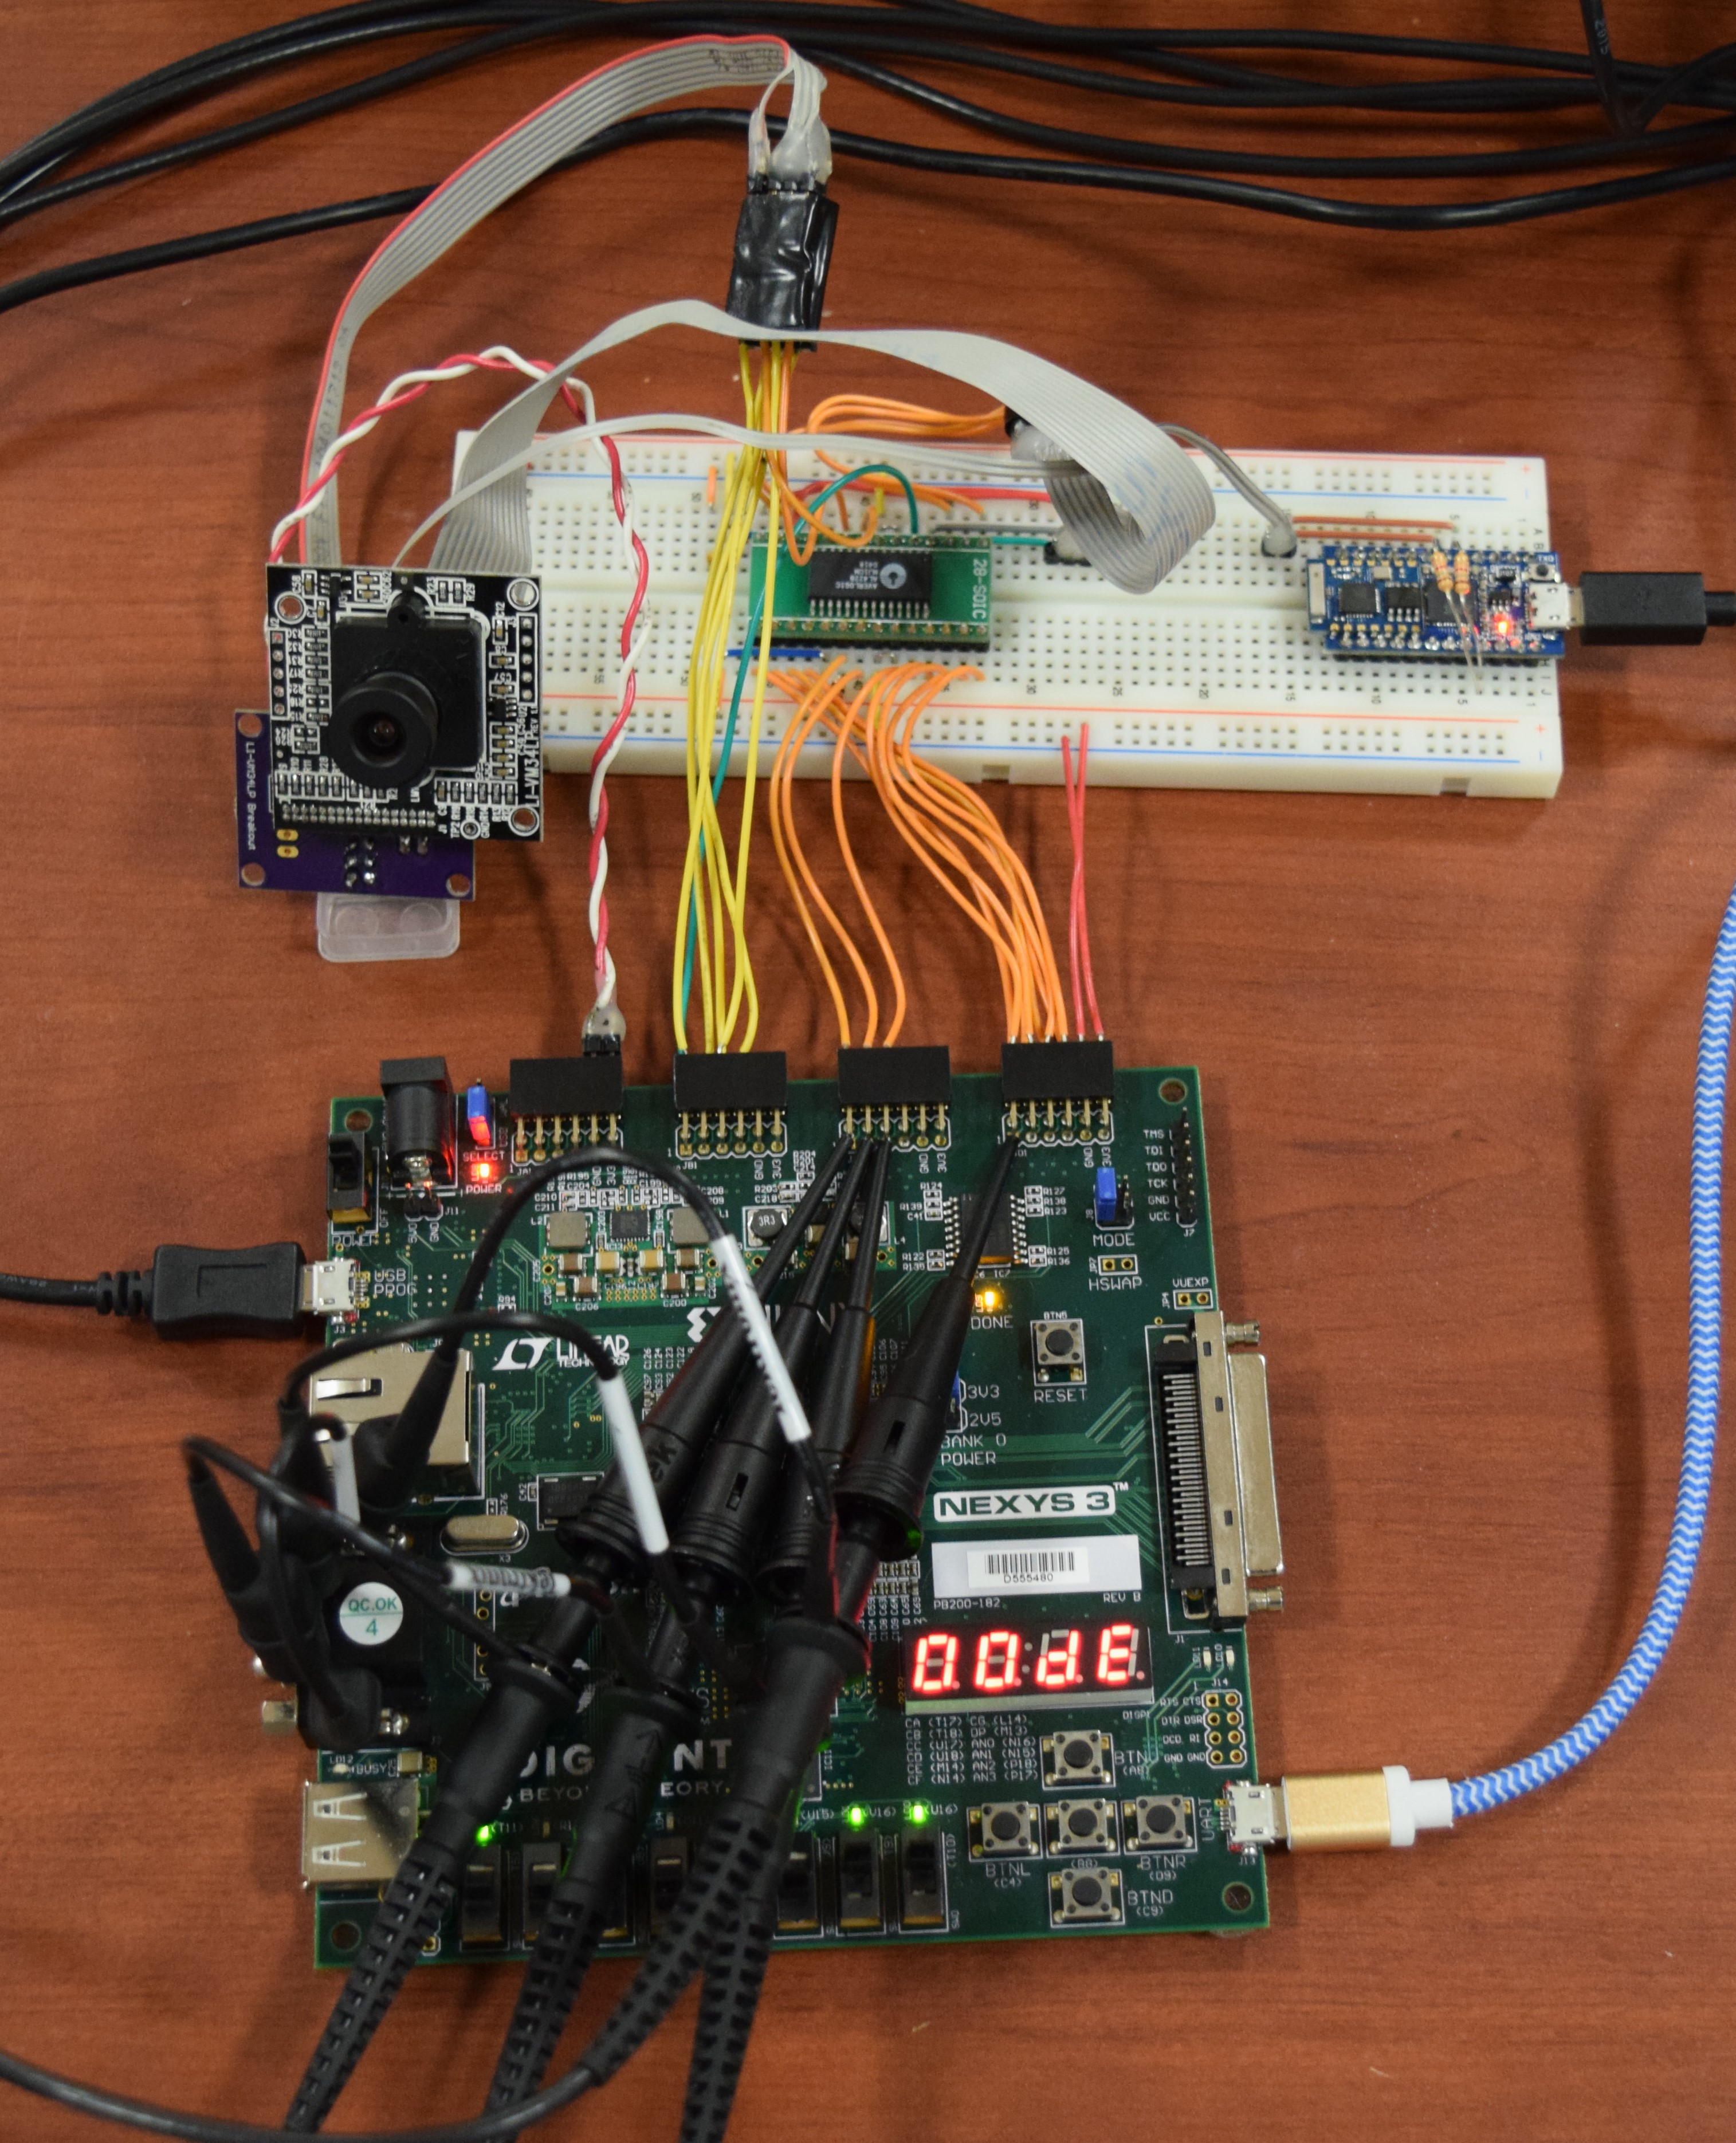
\includegraphics[width=0.75\textwidth]{oScope/camera_fifo/camTestSetup.jpg}}
	\caption{Camera Test Setup}
	\label{camTestSetup}
\end{figure}
